%\subsection{Machine Learning}
% Es un subcampo de l]ecutar dificultosos procesos aprendiendo de datos, en lugar de seguir reglas preprogramadas %\parencite{tec_royal2017machine}.

 %es importante mencionar que existen también cinco tipos de problemas de aprendizaje que se pueden enfrentar: regresión, clasificación, %simulación, optimización y clusterización \parencite{bk_gollapudi2016practical}. Por otro lado, el aprendizaje automático también posee una %división por subcampos que se puede observar en la Figura 14.
%%Figura
% \subsection{Natural Language Processing (NLP)}
 %Naturalmano \parencite{bk_goyal2018deep}. Otra definición para este término implica que es un campo especializado de la informática que es

 %De acuerdo con \citet{bk_goyal2018deep}, e
 
\subsection{Inteligencia Artificial}
La Inteligencia Artificial es el campo de la ciencia informática basada en máquinas que buscan replicar la inteligencia humana, implementando dotes como el razonamiento, aprendizaje y actuar que comúnmente podría hacer un humano \parencite{gl_DEFIA}. La Inteligencia Artificial va más allá que solo la comprensión, sino también el esfuerzo que conlleva construir entidades inteligentes; esto lleva a que su participación en la actualidad esté presente en una gran cantidad de campos, como el aprendizaje y la percepción, como también a campos más específicos como lo es el ajedrez \parencite{bk_russell2004intart}.
\subsubsection{Enfoques de Inteligencia Artificial \parencite{bk_russell2004intart}}
Russell también menciona que la definición de lo que es la Inteligencia Artificial sigue cuatro enfoques, en donde el sistema puede pensar y actuar de forma racional, como también de forma humana: 

\begin{itemize}
	\item \textbf{Actuar como humano:} Alan Turing sugiere una prueba llamada la Prueba de Turing el cual intenta demostrar las pocas diferencias que hay entre un agente inteligente y los seres humanos, ya que menciona que el computador necesita cumplir con seis disciplinas, las cuales son el procesamiento del lenguaje natural, la representación del conocimiento, un razonamiento automático que le permita extraer sus propias conclusiones y un aprendizaje automático que le pueda permitir adaptarse y detectar patrones; además, debe estar dotado con visión computacional y robótica.
	\item \textbf{Pensar como humano:} Considerado como el enfoque del modelo cognitivo, sugiere que el programa debe contar con un mecanismo necesario que le permita determinar cómo piensa un humano, por lo que es necesario penetrar el funcionamiento de dicha mente humana. Para lograr dicha penetración es a través de dos formas, la primera es capturando todos los pensamientos a medida que van apareciendo y la segunda es media una experimentación psicológica.
	\item \textbf{Actuar racionalmente:} Se espera que un agente racional actúe acorde al mejor resultado, o si en caso de que haya incertidumbre, elija la opción que proporcione el mejor resultado esperado. La Prueba de Turing puede permitir realizar dichas acciones racionales.
	\item \textbf{Pensar racionalmente:} Trata de construir sistemas inteligentes que sigan una lógica, el cuál es un esquema de estructuras de argumentación que le permita llegar a una conclusión correcta a partir de premisas correctas.
\end{itemize}
 
\subsection{Aprendizaje Automático}
El Aprendizaje Automático, o Machine Learning (ML) en inglés, forma parte de la rama de lo que es la Inteligencia Artificial, centrando su desarrollo en algoritmos y modelos capaces de  dotar a las computadoras con habilidades que mejoren el rendimiento de realizar una tarea específica sin requerir que sea programada \parencite{pr_diaz}. 

El Aprendizaje Automático utiliza algoritmos que puedan identificar patrones a través de datos almacenados y procesados para la creación de un modelo que le permita realizar análisis predictivos o de detección, ya que busca replicar la inteligencia humana para ser más precisos y mejoren a través de la práctica, siendo adaptable a cualquier escenario en donde los datos puedan cambiar \parencite{gl_azure}.

La aplicación del Aprendizaje Automático es muy amplia, como programas de motores de búsqueda, el diagnóstico automático médico, la detección de fraude en transacciones de una entidad bancaria, análisis de mercado y clasificación de objetos; además del uso de técnicas de reconocimiento facial, voz o escritura \parencite{pr_diaz}.

Existen tres métodos principales de Aprendizaje Automático:
\begin{itemize}
	\item \textbf{Aprendizaje Supervisado:} Se centra en el desarrollo de algoritmos donde interviene un programador para entrenar al modelo qué conclusiones debe hacer mediante un conjunto de datos etiquetados con un resultado ya definido \parencite{gl_oci}.  De esta manera, el modelo puede mapear las entradas con las salidas correctas, mediante una función de pérdida que mida la diferencia entre los verdaderos resultados con el resultado predicho del modelo \parencite{gl_super}. Este modelo puede resolver problemas de clasificación y de regresión, y está presente comúnmente en la detección de fraudes, enfermedades o la predicción del precio. 
	
	\item \textbf{Aprendizaje No Supervisado:} Presenta un enfoque más independiente, donde el modelo aprende a identificar patrones o procesos complejos sin la intervención constante de un programador. Dicho aprendizaje implica un entrenamiento mediante datos no etiquetados y sin un resultado esperado. Este aprendizaje utiliza algoritmos de agrupamiento como k-means, análisis de componentes principales o de asociación, también están en las técnicas de visión computacional. Estos algoritmos tienen como fin realizar grupos o agrupamientos de datos que comparten similitudes, como imágenes, las cuales cada grupo tiene su propia etiqueta \parencite{gl_oci}. 
	
	\item \textbf{Aprendizaje por Refuerzo:} El Aprendizaje por Refuerzo o Recompensa es la retroalimentación que se le da al agente para saber si algo bueno o malo ha ocurrido cuando realiza una acción. Este tipo de aprendizaje está presente en los juegos de ajedrez, donde el refuerzo se realiza cuando finaliza el juego \parencite{bk_russell2004intart}. El agente puede interactuar en un entorno dinámico, tomando decisiones y recibimiento retroalimentación mediante una función de recompensa, con el objetivo de aprender una política, el cual le brinda estrategias de selección para tomar acciones que maximicen el total de recompensas \parencite{gl_cordis}.
	%\medskip
	\begin{figure}[h]
		\begin{center}
			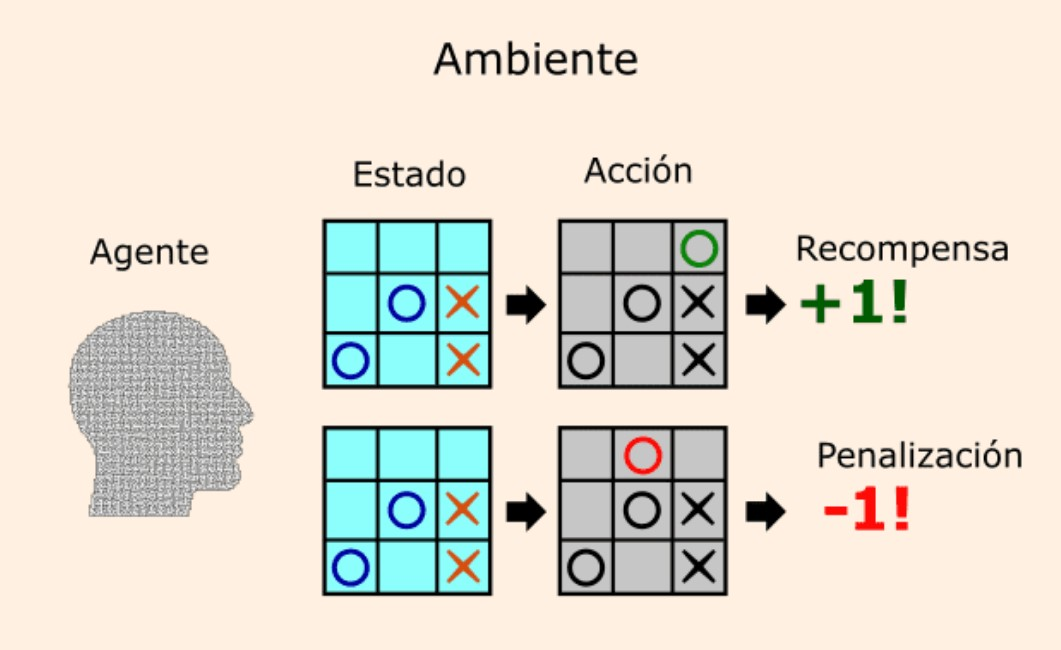
\includegraphics[width=0.65\textwidth]{2/MT/1.jpg}
			\caption{Representación del Aprendizaje por Refuerzo \\
				Fuente: \citep*{gl_ceupe}. \citetitle{gl_ceupe}}
			\label{1:fig2}
		\end{center}
	\end{figure}
	%\medskip
	
	Un concepto fundamental en la que se basa el Aprendizaje por Refuerzo es el Proceso de Decisión de Markov (MDP), el cuál es un marco matemático que le permite realizar un modelo de toma de decisiones en situaciones donde los resultados son aleatorios y depende del control de quien toma las decisiones. Como se muestra en la Figura \ref{1:mark},, este es un ejemplo simple de MDP, el cuál en cada paso de tiempo, el proceso inicia en un estado $S$, y el que toma la decisión puede elegir una acción a que está disponible en dicho estado. El resultado de esto otorga un nuevo estado $St$ y una recompensa $Ra (S, St)$ \parencite{gl_markov}.
	%\medskip
\begin{figure}[h]
	\begin{center}
		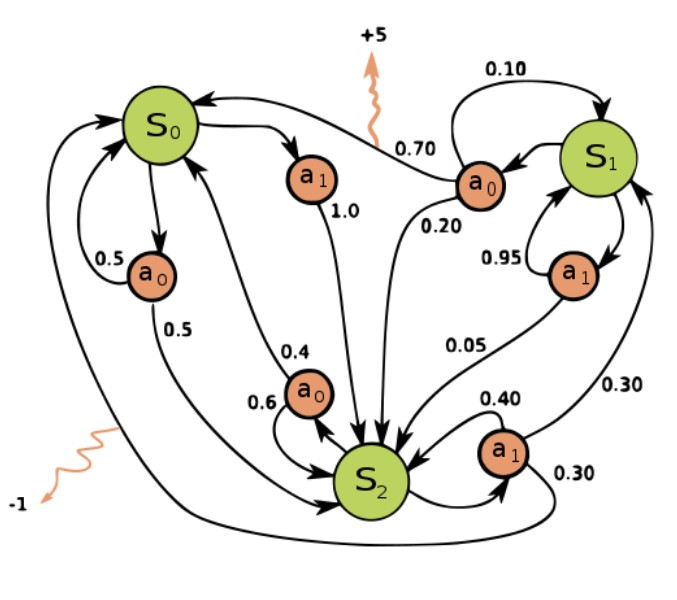
\includegraphics[width=0.65\textwidth]{2/MT/2.jpg}
		\caption{Proceso de decisión de Markov \\
			Fuente: \citep*{gl_markov}. \citetitle{gl_markov}}
		\label{1:mark}
	\end{center}
\end{figure}
%\medskip

Para que el MDP pueda conocer las probabilidades o dichas recompensas, se define una función el cuál es conocido como Q-learning:
%\medskip
\begin{equation} 
Q(s,a) = \sum_{s^{t}}P_{a}(s,s^{t})(R_{a}(s,s^{t})+\gamma V(s^{t}))
\end{equation}
%\medskip
Donde $P_{a}$ es la probabilidad de que la acción a en el estado $s$ en un tiempo determinado de un nuevo estado $s^{t}$, el $R_{a}$ es la recompensa esperada que recibirá de pasar un estado a otro debido a la acción $a$. Mientras que el $V$ contiene los valores reales del nuevo estado \parencite{gl_markov}.

\end{itemize}
\subsection{Aprendizaje Profundo}
Los algoritmos de aprendizaje profundo forman parte del aprendizaje automático, y los cuáles han tomado una mayor participación en los últimos años por la alta disponibilidad de grandes datos y los recursos computacionales potentes. Debido a que se cuenta con GPUs más rápidas para el entrenamiento de grandes modelos profundos, los algoritmos de Aprendizaje Profundo supera a los modelos tradicionales en múltiples aplicaciones, como el mejoramiento del rendimiento de modelos de reconocimiento de imágenes, redes neuronales convolucionales profundas al reducir la tasa de error, el rendimiento de sistemas de reconocimiento de voz el cual estuvo estancado varios años; y también aporta enormemente en el campo de la investigación del Procesamiento del Lenguaje Natural (NLP) \parencite{bk_grafo}.

\subsubsection{Redes Neuronales Profundas (DNN)}

Las Redes Neuronales Profundas, o Deep Neural Network en inglés, permiten al modelo mediante su entrenamiento a realizar tareas más complejas que son difíciles de hacer utilizando redes neuronales tradicionales. Asimismo, dichas redes se inspiran del cerebro humano, teniendo un diseño que no solo se limita a seguir reglas establecidas, sino también predecir y sacar conclusiones \parencite{gl_bot}. Las Redes Neuronales Profundas si bien son similares a las Redes Neuronales Tradicionales, el término de “Profundo” hace referencia al número de capas ocultas que forma parte de la red, teniendo más nodos de procesamiento, las cuáles son conocidas como neuronas \parencite{gl_edutech}.
    
%\medskip
\begin{figure}[h]
	\begin{center}
		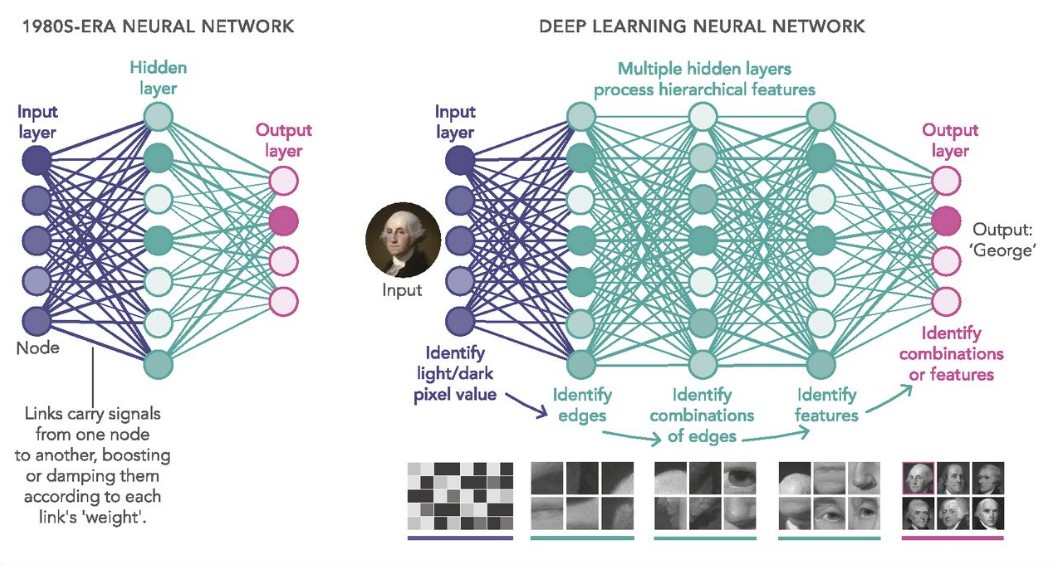
\includegraphics[width=0.65\textwidth]{2/MT/3.jpg}
		\caption{Comparación entre una Red Neuronal Artificial y una Red Neuronal Profunda \\
			Fuente: \citep*{gl_compara}. \citetitle{gl_compara}}
		\label{1:fig2}
	\end{center}
\end{figure}
%\medskip

Este tipo de red está presente en el reconocimiento de voz, sonidos y grafos, además que utilizan “Big Data” para la resolución de problemas en la que la intervención humana es limitada \parencite{gl_bot}. 


\subsection{Aprendizaje Profundo por Refuerzo (DRL)}
El Aprendizaje Profundo por Refuerzo o Deep Reinforcement Learning (DRL) es la combinación entre técnicas de Redes Neuronales Profundas con Aprendizaje por Refuerzo, esto tiene como beneficio la interacción de forma iterativa en un entorno para tomar decisiones que busquen maximizar una función de recompensas para encontrar estrategias más sofisticadas \parencite{gl_geekrein}. El Aprendizaje Profundo por Refuerzo es un paso importante en la evolución del aprendizaje de las máquinas que toma la decisión más beneficiosa y que utiliza esa decisión en escenarios futuros \parencite{gl_iic}.
%\medskip
\begin{figure}[h]
	\begin{center}
		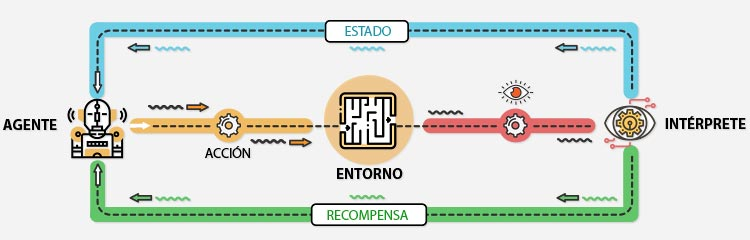
\includegraphics[width=0.65\textwidth]{2/MT/4.jpg}
		\caption{Componentes que conforma el Aprendizaje por Refuerzo \\
			Fuente: \citep*{gl_iic}. \citetitle{gl_iic}}
		\label{1:fig2}
	\end{center}
\end{figure}
%\medskip

 Un modelo de Aprendizaje Profundo por refuerzo está conformado por un agente, el cual es el que aprende las reglas a seguir y toma decisiones mediante la interacción con el entorno utilizando técnicas de Redes Neuronales Profundas.  Se menciona, además, que el DRL está basado en Q-learning, componentes de políticas para que se diriga las decisiones del agente, conceptos claves como lo son la función de valor que calcula las recompensas, las cuales son una señal que muestra el entorno sobre la acción deseada para que el agente cambie el estado de la situación actual del entorno. Son ampliamente utilizados en los sistemas de navegación, tratamientos médicos como la recomendación de medicamentes, perfeccionar los diseños de materiales con el fin de aumentar su efectividad y la personalización del entorno de eCommerce según los gustos de cada cliente \parencite{gl_iic}.
 
Con lo que respecta a los sistemas de navegación, se aplican tecnologías de información avanzadas para hacer frente al problema del control adaptativo de las señales de tráfico. Existen muchas investigaciones y propuestas como un enfoque que realiza simulaciones con datos de tráfico reales de la ciudad de Toronto, donde los agentes se coordinan mediante intersecciones vecinas. También la integración de un algoritmo de Aprendizaje por Refuerzo multiagente para enfrentar a los desafíos de estacionariedad y dimensionalidad en el control adaptativo de las señales de tráfico \parencite{pr_artiDeep}.

\subsubsection{Deep Q-Network (DQN)}
Para que el modelo de Aprendizaje Profundo por Refuerzo pueda aprender, es fundamental tener una función de valor. Esta función está presente en las arquitecturas DQN, la cuál nace en el año 2015 por DeepMind \parencite{pr_artiDeep}. Este algoritmo es creado por la necesidad de afrontar la inestabilidad de aprendizaje de la combinación de RL con redes neuronales, ya que almacena todo lo aprendido por el agente y luego lo reproduce aleatoriamente para proporcionar datos de entrenamiento diverso y des correlacionados \parencite{gl_DeepMind}. 

%\medskip
\begin{figure}[h]
	\begin{center}
		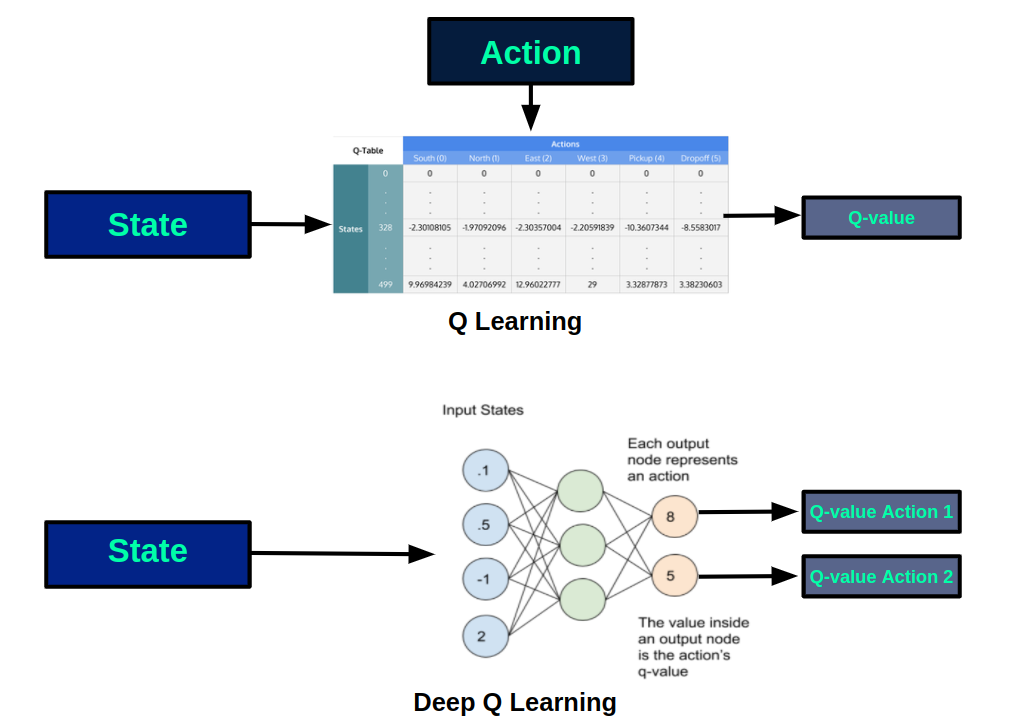
\includegraphics[width=0.65\textwidth]{2/MT/5.png}
		\caption{Diferencias entre Q-Learning y Deep Q-Learning \\
			Fuente: \citep*{gl_Damavis}. \citetitle{gl_Damavis}}
		\label{1:fig2}
	\end{center}
\end{figure}
%\medskip

Este algoritmo ha presentado varios avances, estabilizando la dinámica de aprendizaje, priorizando las experiencias que ya han sido aprendidas o también conocidas como Experience Replay, además de normalizar, agregar y reescalar los resultados \parencite{gl_DeepMind}. 

\subsubsection{Política}

Una política es aquella que busca un mapeo óptimo en las acciones realizadas por los estados. Uno de los algoritmos de una política es el algoritmo de actor-crítico que aprende una función de valor de estado para actualizarlo a partir de estimaciones posteriores para reducir la varianza y acelerar el aprendizaje. Además de esto, en el campo de Aprendizaje por Refuerzo y Aprendizaje Profundo por Refuerzo, se tiene un enfoque en el gradiente de política y su optimización, donde el método más popular es el REINFORCE, que en comparación al Q-learning que es más eficiente en el uso de los datos, este tiende a ser más estable. Existen también otras gradientes que son eficientes en situaciones donde las acciones son continuas, una de estas gradientes es la Gradiente de Política Determinista (DPG), el cual se basa en la estimación de la gradiente de la función de valor de acción, siendo más eficiente que los métodos estocásticos de gradiente de política, además, utiliza Redes Neuronales Profundas para una mayor estabilidad del modelo de aprendizaje \parencite{pr_artiDeep}.

Para la optimización de las políticas, se utiliza el método Trust Region Policy Optimization (TRPO), que controla las actualizaciones de la política mediante la restricción de región de confianza, mejorando la estabilidad del modelo y la eficiencia computacional \parencite{pr_artiDeep}. 

\subsubsection{Recompensa}
Las recompensas son las que proporcionan una retroalimentación al agente para la toma de decisiones. Esta recompensa es calculada mediante una función que es modificada para facilitar el aprendizaje mientras se obtiene una política óptima. Sin embargo, estas funciones de recompensas no suelen estar presente en mucho de los problemas, por lo que se recurre al aprendizaje por imitación, donde el agente aprende mediante demostraciones de expertos \parencite{pr_artiDeep}. Este tipo de aprendizaje tiene dos enfoques los cuáles son:

\begin{itemize}
	\item \textbf{Deep Q-learning from Demonstrations (DQfD):} Este enfoque combina pérdidas por diferencia temporal (TD), supervisadas y regularizadas. Es entrenado a partir de datos de demostración con el fin de establecer una función de valor y así generar sus propias muestras para el entrenamiento del modelo.
	\item \textbf{Inverse Reinforcement Learning (IRL):} Permite aprender políticas a partir de los datos, evitando aprender una función de recompensa.
\end{itemize}

\subsubsection{Modelo y Planificación}
El entorno es un modelo que incluye el modelo de transición y un modelo de recompensa, este enfoque de Aprendizaje por Refuerzo basados en Modelos puede aprender de manera eficiente la función de valor y política, teniendo una ventaja al Aprendizaje por Refuerzo sin modelo, ya que no requiere de un gran número de muestras; sin embargo, puede tener problemas a la hora de identificar los modelos estimados y teniendo como resultado que no sean precisos o que el rendimiento sea limitado. Para hacer frente a este problema, la planificación construye una función de valor o una política en base a un modelo \parencite{pr_artiDeep}.

\subsubsection{Exploracion}
Para reducir la incertidumbre sobre la función de recompensa y las probabilidades del entorno, el agente utiliza la exploración como principal herramienta de apoyo. La incertidumbre se puede cuantificar como intervalos de confianza o los propios parámetros del entorno relacionados con el recorrido de estado-acción. Existe más de un enfoque de exploración, como lo es la exploración basada en recuentos de recorridos para guiar el comportamiento del agente con el fin de reducir la incertidumbre, también está el enfoque de la motivación intrínseca que explora solo lo que es más sorprendente en un proceso de aprendizaje basado en los cambios en el error de la predicción \parencite{pr_artiDeep}.

\subsection{Fundamentos de grafos}
Los grafos son la representación que existe en la relación entre entidades, y que están presentes en varios campos como las ciencias sociales, química, biología y física. Un ejemplo de estos grafos en el campo de la química son los compuestos químicos, en donde los átomos representan los nodos y los enlaces químicos representan las aristas \parencite{bk_grafo}.

Un grafo puede ser denotado como $G = \{V, E\}$, donde $V = \{v_{1}, . . ., v_{N}\}$ es un conjunto de $N = |V|$ nodos y $E = \{e_{1}, . . . e_{M}\}$ es un conjunto de $M$ aristas, además, $G$ representa el tamaño que tiene el grafo. Un aspecto esencial en los grafos son los nodos, los cuales representan a las entidades mientras que el conjunto de aristas representa las conexiones que existen entre los nodos. Existen dos tipos de grafos, los dirigidos donde las aristas van en orden, es decir desde el nodo 1 al nodo 2, mientras que los no dirigidos el orden de los dos nodos no altera el resultado, ya que puede ir del nodo 2 al nodo 1 y viceversa, sin tener diferencias \parencite{bk_grafo}.

%\medskip
\begin{figure}[h]
	\begin{center}
		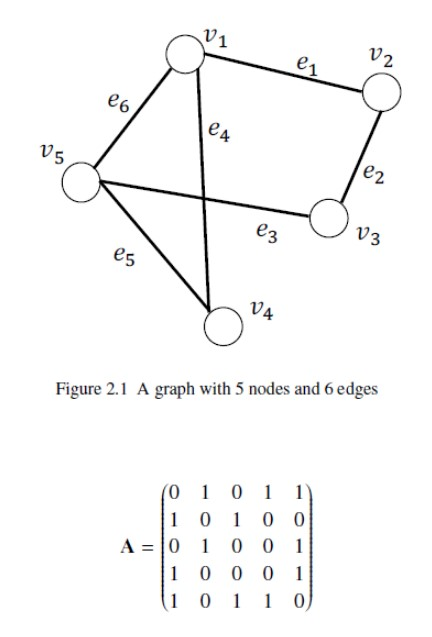
\includegraphics[width=0.5\textwidth]{2/MT/6.jpg}
		\caption{Propiedades u medidas de un grafo \\
			Fuente: \citep*{bk_grafo}. \citetitle{bk_grafo}. (p. 19)}
		\label{1:fig2}
	\end{center}
\end{figure}
%\medskip

Otro aspecto que conforma un grafo es su Matriz de Adyacencia, el cual se denota como $A \in \{0, 1\}$$NxN$. Cada $A_{ij}$ representa la relación que hay entre dos nodos. Cabe mencionar que, en un grafo no dirigido, su matriz de adyacencia es simétrica, es decir, $A_{ij} = A_{ji}$  \parencite{bk_grafo}.


\subsubsection{Propiedades de un grafo \parencite{bk_grafo}}
El grado indica la cantidad de veces que un nodo está conectado a otro, el cual puede ser calculado de la siguiente forma:
%\medskip
\begin{equation} 
	d(v_{i}) = \sum_{v_{j}\in V }\mathbb{I}_{\varepsilon}(\left \{v_{i},v_{j}  \right \}) ,
\end{equation}
%\medskip

\begin{equation} 
	\mathbb{I}_{\varepsilon}(\left \{v_{i},v_{j}  \right \}) = \begin{Bmatrix}
		1\;\;\;\; \textrm{if}\;  (v_{i},v_{j}) \in \varepsilon, \\ 
		0\;\;\;\; \textrm{if}\;  (v_{i},v_{j}) \notin \varepsilon
	\end{Bmatrix}
\end{equation}
%\medskip
El grado también puede ser calculado mediante su matriz de adyacencia de la siguiente forma:
%\medskip

\begin{equation} 
	d(v_{i}) = \sum_{j = 1}^{N}A_{i,j}
\end{equation}
%\medskip
En contraste al grado, los vecinos son el conjunto de nodos que están conectados a un nodo. El camino de un grafo es el recorrido que hay entre los nodos y las aristas y su longitud es el número de aristas que existen. En este camino, se forman rastros que son aristas distintas y la trayectoria que son los nodos distintos. Para que haya conectividad, se necesita al menos que haya un camino entre cualquier par de nodos. Para hallar el camino más corto, se calcula de la siguiente manera:
%\medskip

\begin{equation}
	p_{st}^{sp} = arg \min_{p\in p_{st}}\left | p \right |
\end{equation}
%\medskip

Donde $p$ es el camino en $p_{st}$ con su longitud.
Para calcular el diámetro de un grafo, es de la siguiente manera:
%\medskip

\begin{equation}
	diameter(G) = \max_{v_{s},v_{t}\in V}\min_{p\in P_{st}}
\end{equation}
%\medskip


\subsubsection{Procesamiento de señales de Grafos \parencite{bk_grafo}}

Las señales de grafos son las características o atributos asociados en cada nodo, los cuales almacenan la conectividad o estructura de los nodos, como también sus datos. Esta señal consiste en un grafo y una función de mapeo donde se le asigna los valores reales correspondiente a los nodos, el cual es representado de la siguiente manera:
%\medskip

\begin{equation}
	f: V \rightarrow \mathbb{R}^{Nxd}
\end{equation}
%\medskip

Donde $d$ es el vector (dimensión del valor) que está asociado a cada nodo.


\subsubsection{Transformación de Fourier en Grafos (GFT) \parencite{bk_grafo}}
En comparación a la clásica transformación de Fourier, que realiza un análisis de señales establecidas en la dimensión del tiempo o espacio, esta extensión realiza el análisis en la dimensión de un grafo, con el fin de descomponer dicha señal en una serie de componentes espectrales basados en los autovectores de la matriz Laplaciana del grafo, la cual es una matriz que captura la estructura del grafo con el fin de realizar diversas operaciones y análisis. Dicha Matriz Laplaciana ($L$) es la diferencia de la matriz diagonal de los grados ($D$) y la matriz de adyacencia del grafo ($A$). 

La Transformación de Fourier en grafos se puede definir matemáticamente de la siguiente manera: 

%\medskip

\begin{equation}
	f[i] = \sum_{l=1}^{N}\hat{f}[l]u_{l}[i]
\end{equation}
%\medskip

Donde: 

$\hat{f}[l]$ es el l-ésimo coeficiente de Fourier en grafos.

$u_{l}$ es el l-ésimo autovector de la matriz Laplaciana $L$ del grafo.

\subsubsection{Tipo de Grafos \parencite{bk_grafo}}

\begin{itemize}
	\item \textbf{Grafos Heterogéneos:} Son los grafos más simples explicados en los anteriores puntos, en donde solo tienen un tipo de nodos y aristas.
	
	\item \textbf{Grafos Multidimensionales:} Este tipo de grafo puede compartir múltiples relaciones en simultáneo entre un par de nodos, como por ejemplo cuando los usuarios de YouTube, considerados como nodos, pueden suscribirse entre ellos, donde cada tipo de relación se considera como una dimensión.
	
	\item \textbf{Signed Graphs:} Este tipo de grafo contiene tanto aristas positivas como negativas, y son popularmente representados en las plataformas sociales en línea, como, por ejemplo, cuando un usuario puede bloquear o dejar de seguir a otros usuarios, dicha acción de seguir o no seguir pueden considerarse como las aristas positivas y negativas, respectivamente.
	
	\item \textbf{Hypergrafos:} Este tipo de grafo en comparación a los anteriores, este no solo tiene información entre pares de aristas, ya que, en el mundo real, estas relaciones van más allá que las asociaciones entre pares, como por ejemplo los artículos publicados por un autor.
	
	\item \textbf{Dynamic Graph:} Es un tipo de grafo en el cual sus conexiones entre los nodos pueden cambiar con el tiempo, reflejando un comportamiento y evolución continua entre estos.
	
\end{itemize}


\subsection{Métodos de Redes Neuronales Profundas basadas en Grafos}
\subsubsection{Graph Neural Networks \parencite{bk_grafo}}

Las Redes Neuronales Gráficas (GNNs) son métodos que aplican Redes Neuronales Profundas a datos estructurados representados en grafos. Este método puede ser representado como un proceso de aprendizaje de representación en grafos y que están enfocados en aprender las características representativas de cada nodo con el fin de facilitar las tareas del grafo. Dicho proceso se puede representar de la siguiente manera:

%\medskip

\begin{equation}
	F^{(of)}= h(A,F^{^{(if)}})
\end{equation}
%\medskip

Donde $A$ representa la matriz de adyacencia del grafo con $N$ nodos y $F^{^{(if)}}$ y $F^{^{(of)}}$ representan las matrices de características de entrada y salida, las cuales también tienen las dimensiones  del grafo. Los subíndices “$if$” y “$of$” son los filtros que se realizan dentro del grafo y que en la figura está representada el proceso tradicional de filtrado del grafo a sus características de los nodos:

%\medskip
\begin{figure}[h]
	\begin{center}
		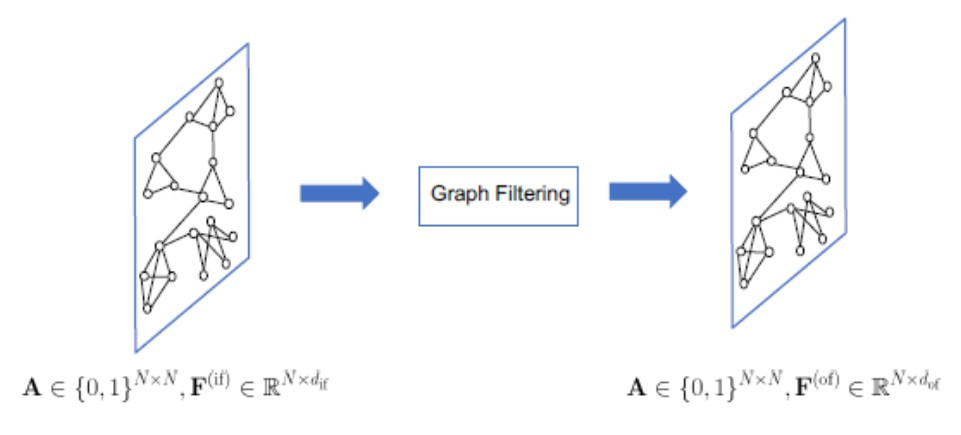
\includegraphics[width=0.75\textwidth]{2/MT/7.jpg}
		\caption{Operación de filtración de grafos \\
			Fuente: \citep*{bk_grafo}. \citetitle{bk_grafo}. (p. 108)}
		\label{1:fig2}
	\end{center}
\end{figure}
%\medskip


Existen otras operaciones que son necesarias para las tareas centradas en grados y generalmente son operaciones de agrupación a partir de las características de los nodos. Este proceso de agrupación toma un grafo como entrada y luego producen un grafo reducido con pocos nodos, como se observa en la siguiente figura:

%\medskip
\begin{figure}[h]
	\begin{center}
		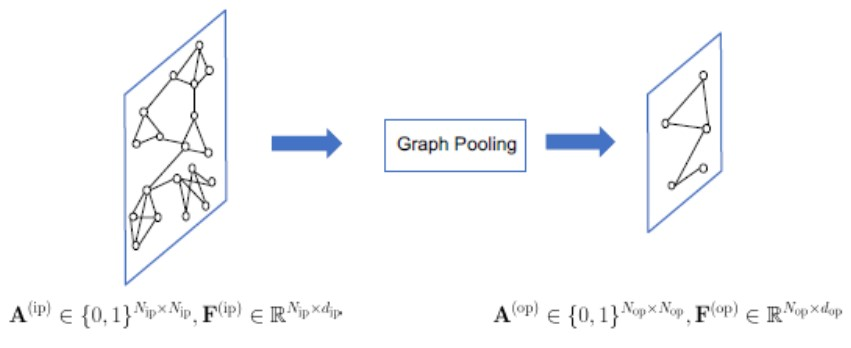
\includegraphics[width=0.75\textwidth]{2/MT/8.jpg}
		\caption{Operación de filtración de grafos \\
			Fuente: \citep*{bk_grafo}. \citetitle{bk_grafo}. (p. 109)}
		\label{1:fig2}
	\end{center}
\end{figure}
%\medskip

Dicha operación se puede describir de la siguiente manera:

%\medskip

\begin{equation}
	A^{(op)},F^{(op)}= pool(A^{^{(ip)}},F^{^{(ip)}})
\end{equation}
%\medskip
Los subindices $ip$ y $op$ indican la entrada y salida de la agrupación.



\subsubsection{Robust Graph Neural Networks}
Al igual que las DNNs tradicionales, estas son vulnerables a ataques adversarios, generando perturbaciones en la manipulación de la estructura del grafo y la características de los nodos para engañar a los modelos de GNNs. Por esta limitación, Robusta Graph Neural Networks es una extensión de las GNNs que adoptan medidas críticas de seguridad, las cuáles pueden estar presentes en los sistemas financieros y la gestión de riesgo. La RGNNs comunmente utiliza un enfoque de limpieza del grafo perturbado, los cuáles han sido victimas de una violación de ciertas propiedades que presenta el grafo real \parencite{jin2020graph}.


\subsubsection{Scalable Graph Neural Networks}
Las GNNs tradicionales presentan problemas de escalabilidad que impide la adopción de grados a gran escala, debido a que utiliza un método de gradiente para minimizar la función de pérdida en cada etapa de representación de nodos, requiriendo una gran cantidad de recursos computacionales y operaciones de cálculos (Libro). Para abordar dichos problemas, se utilizan las técnicas y enfoques de las SGNNs para que las GNNs sean más eficientes a medida que el tamaño y la complejidad de los grafos van aumentando. Una de las principales técnicas de las SGNNs es el Graph Coarsening que utiliza la reducción de grafos para el entrenamiento escalable de estas \parencite{huang2021scaling}.

